\documentclass{llncs}

\usepackage[cp1250]{inputenc}  % or [cp1250], or [latin2], or whatever
                               % suitable for your system
\usepackage{graphicx}
\usepackage{url}

\newcommand{\keywords}[1]{\par\addvspace\baselineskip
\noindent\keywordname\enspace\ignorespaces#1}


\begin{document}

\mainmatter  % start of an individual contribution

\title{Web Semantization}
%\titlerunning{Web Semantization}


\author{Jan Dedek\inst{1} \and Alan Eckhardt\inst{1,2} \and Leo Galambos\inst{1} \and Peter Vojt�\inst{1,2}}

\institute{Charles University, Faculty  of  Mathematics  and  Physics, Prague, Czech Republic \email{\{dedek, eckhardt, galambos, vojtas\}@ksi.mff.cuni.cz}
\and Academy of Sciences of the Czech Republic, Institute of Computer Science}


%\institute{Charles University in Prague, Department of software engineering,\\
%Malostranske namesti 25, Prague, Czech Republic}%\\
%}



%\authorrunning{Vojtas et al.}

%       \affaddr{Charles University in Prague}\\
%       \affaddr{Malostranske namesti 25 }\\
%       \affaddr{Prague, Czech Republic}\\
%       \email{jan.dedek@mff.cuni.cz}
%\alignauthor Alan Eckhardt\\
%       \affaddr{Institute of Computer Science, Academy of Sciences of the Czech Republic}\\
%       \affaddr{Pod Vodarenskou vezi 2}\\
%       \affaddr{Prague, Czech Republic}\\
%       \email{eckhardt@cs.cas.cz}
%\alignauthor Peter Vojtas\\
%       \affaddr{Institute of Computer Science, Academy of Sciences of the Czech Republic}\\
%       \affaddr{Pod Vodarenskou vezi 2}\\
%       \affaddr{Prague, Czech Republic}\\
%       \email{vojtas@cs.cas.cz}
%}
%\additionalauthors{Additional author: Leo Galambos (Department of software engineering,
%Charles University in Prague, Czech Republic,
%email: {\texttt{leo.galambos@mff.cuni.cz}}).}

\maketitle


\begin{abstract}
%In this paper we developed the idea of web semantization, which can help to arch over the gap between the web of today and the Semantic web.
Web Semantization is a concept we introduce in this paper. We understand Web Semantization as an automated process of increasing degree of semantic content on the web. Part of content of the web is further usable, semantic content (usually annotated) is more suitable for machine processing.
The idea is supported by models, methods, prototypes and experiments with a web repository, automated annotation tools producing third party semantic annotations, semantic repository serving as a sample of semantized web and a proposal of an intelligent software agent. We present a proof of concept that even today it is possible to develop a semantic search engine designed for software agents.
\keywords{Web Content Mining, Web Content Machine Processing, Annotation, Linguistic Analysis}
\end{abstract}

\section{Introduction}
In their Scientific American 2001 article \cite{biblio:2001-Berners-Lee-SemanticWeb}, Tim Berners-Lee, James Hendler and Ora Lassila unveiled a nascent vision of the semantic web: a highly interconnected network of data that could be easily accessed and understood by a desktop or handheld machine. They painted a future of intelligent software agents that would ``answer to a particular question without our having to search for information or pore through results'' (quoted from \cite{biblio:feigenbaum_semantic_2007}). Lee Feigenbaum, Ivan Herman, Tonya Hongsermeier, Eric Neumann and Susie Stephens in their Scientific American 2007 article \cite{biblio:feigenbaum_semantic_2007} conclude that ``Grand visions rarely progress exactly as planned, but the Semantic Web is indeed emerging and is making online information more useful as ever''. L. Feigenbaum et al. support their claim with success of semantic web technology in drug discovery and health care (and several further applications). These are mainly corporate applications with data annotated by humans. Ben Adida when bridging clickable and Semantic Web with RDFa (\cite{biblio:AdidaClickable}) assumes also human (assisted) activity by annotations of newly created web resources. \par

But what to do with the content of the web of today or of pages published without annotations? The content of the web of today is too valuable to be lost for emerging semantic web applications. We are looking for a solution how to make it accessible in semantic manner. \par

In this paper we would like to address the problem of semantization (enrichment) of current web content as an automated process of third party annotation for making at least a part of today's web more suitable for machine processing and hence enabling it intelligent tools for searching and recommending things on the web (see \cite{biblio:LeeWebThings}). \par

Our main idea is to fill a semantic repository with information that is automatically extracted from the web and make it available to software agents. We give a proof of concept that this idea is realizable and we give results of several experiments in this direction.

Our web crawler (see Fig.\ref{img:Semantization}) downloads a part of the web to the web repository (Web Store). Resources with semantic content can be uploaded directly to the semantic repository (Semantic Store). Extractor~1 (classifier) extracts those parts of Web Store which are suitable for further semantic enrichment (we are able to enrich only a part of resources). More semantic content is created by several extractors and annotators in several phases. The emphasis of this paper is on the automation and the usage of such extracted/enriched data.

\begin{figure}
\centering
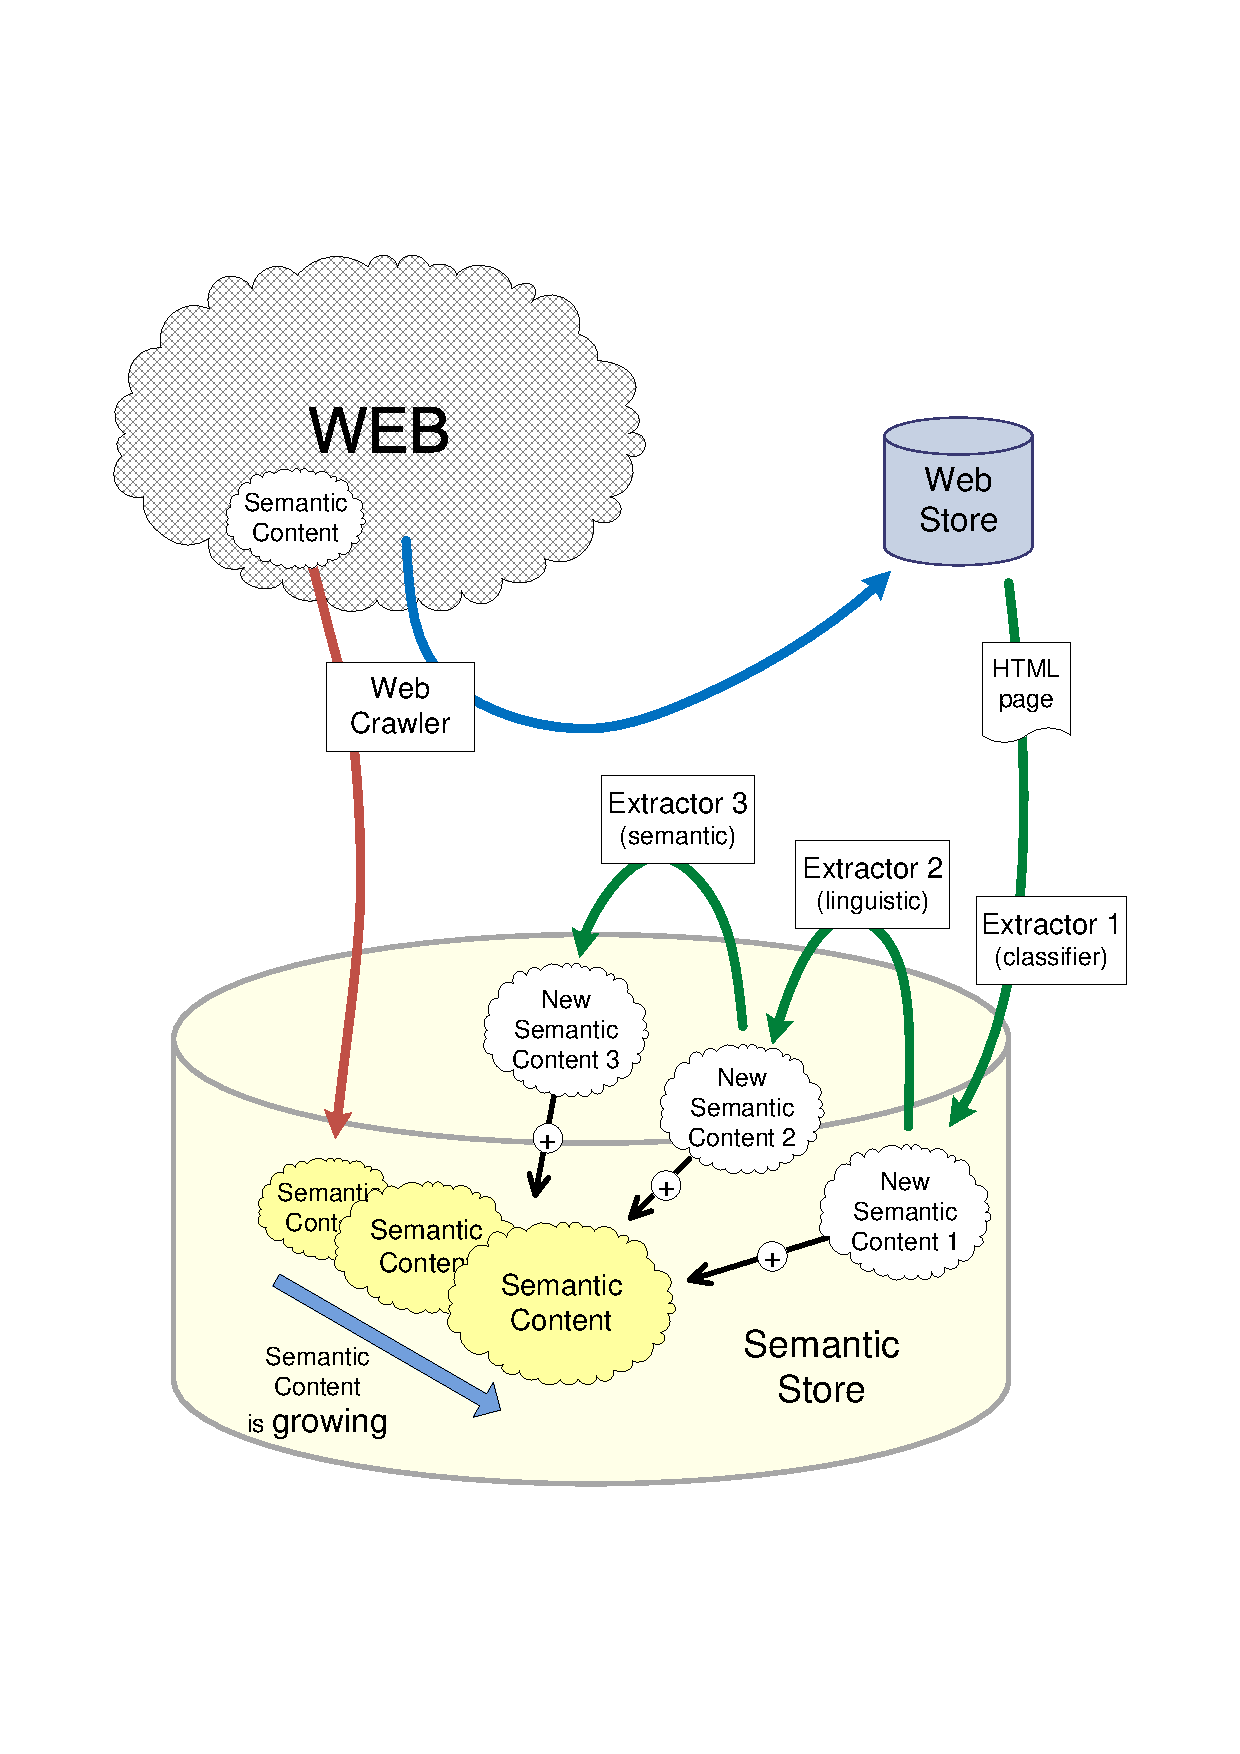
\includegraphics[height=.8\hsize, width=\hsize]{img/Semantization}
\caption{The process of semantization of the Web}
\label{img:Semantization}
\end{figure}


%\subsection{Motivation example}

%Our motivation example aims to illustrate a possible use of such a semantized web by an intelligent agent. Imagine a user wanting to buy a car. She has special requirements on car properties (possibly containing conflicting objectives as price and consumption) and its safety when used in Czech Republic (she knows about the increase of traffic accidents after unification of Germany, when fast western cars crashed on narrow roads of eastern part often \textbf{[6??]}).  Information about car properties can be extracted from several web shop pages typically in tables. Information about involvement in traffic accidents and if involved, then of injury rate, are hidden e.g. in textual traffic accidents reports of regional fire department (in Czech Republic responsible for emergency recovery). Our semantic store contains these information annotated (by possibly several tools) also by uncertainty of extraction and/or annotation process. Our intelligent agent can aggregate these (often conflicting) information and offer user best (top-k) answers according to a user dependent equilibrium between car properties, safety and reliability and/or (un)certainty of this information.

%\subsection{Our contributions}

%Our main contribution is the proof of concept of the idea of semantization of the web of today as an automated process making it ready for intelligent machine search. Particular contributions consists of models, methods and tools of :

%\begin{itemize}
%\item web repository based on highly efficient web crawler and a repository with extended soft computing classification (search) capabilities (see chapter 4??); 
%\item automated domain independent intermediate annotation of suitable pages from our web repository with soft computing heuristics (see chapter 5??);
%\item automated domain dependent annotation with extraction ontology and ILP learning from similar repeating structured linguistic data (see chapter 6??); 
%\item Semantic repository serving as a sample of semantized web, extension of the ontology model for additional annotation (e.g. uncertainty annotation) (see chapter 7??)
%\item Intelligent agent using soft computing tools for matching user preferences (see chapter 8??).
%\end{itemize}
%



%\section{Where is the problem with semantization of the Web of today?}

%Web of today contains lot of valuable information which is worth of being subject of intelligent search (also archived non-existing pages, e.g. http://www.archive.org/index.php and http://www.searchengineshowdown.com/others/archive.shtml ). Main obstacle is that these resources are designed for human consumption and are hardly understandable for a machine. The size of these resources excludes human search. Using traditional search engines has limited capabilities. One solution is to semantically enrich these pages (semantize) and make them machine processable.  As it is not an easy task, the problem is who will do it and why. This is well under way for new corporate applications and publishers willing to annotate their resources and the driver can be better services (and higher profit, faster emergency warning, ... \textbf{[3??]}).

%A step in direction of semantic enrichment is presented also by indexes of various search engines - they represent a certain sort of semantic enrichment. The problem is that those indexes are not available for writing own applications. Moreover search engines of today fail in linguistic search. Fixed page rank prohibits one to find relevant pages which are not highly quoted (e.g. traffic accident reports). Web shops enable only conjunctive query search. Web shops are mainly classified as hidden web, and are hard for machine processing. Survey pages can usually find cheapest item (when you know what you want). Linguistic search engines are just starting to be developed, mainly with some narrow focus. Another step to semantic enrichment are different WIE - 

%Web Information Extraction tools, nevertheless they do not annotate sources, From our point of view, we see the main problem of current tools with own enrichment of web content is that this enrichment mostly serves query answering and does not produce annotation of sources accessible for public for further processing.
%When we understand semantization (of the web of today) as a semantic enrichment automatically producing semantically annotated resources for further (third party) machine processing, then main problems of semantic enrichment of the web are:
%\\- How to do it automatically, in which order, which pages should be enriched first, \dots? Do the enrichment in the time of query or in advance?
%\\- Where to store such enriched (annotated) pages?
%\\- With respect to which ontology to make annotation?
%\\- What are metrics of satisfactory semantic enrichment?
%\\- When done, how to use it? Current RDF querying languages are not very promising for intelligent search.
%\\- How to achieve reusability/social web - agent once trained can be used by other user (with changed user preferences)
%\\- Which extractors are trustworthy; which URLs to search (Czech car offers)
%\\- User friendly - no need to search by keyword, only user preferences input.
%\\- Automation - when a new offer emerges on a page, extractor captures the information, stores it in the semantic store and agent has always information up-to-date.
%\\- When one extractor misses an attribute value, another can find it and store it. Such an automated semantic enrichment will be error prone. How to represent uncertainty? Problem of complete information?
%







\section{Idea of Web semantization}
%Here we would like to present the idea of our contribution to web semantization.

\textbf{First idea is the idea of a web repository.} It develops as follows in details. Semantic enrichment is in fact a data mining task (although a special one) - to add to web documents a piece of knowledge, which is obvious for human perception not for a machine. That means to annotate data by concepts from an ontology which is the same as to map instances to ontology. Such a data mining task will be easier to solve when there is a sort of a repetition (modulo some similarity).\par 
We decided to enrich only textual content for the present, no multimedia (this substantially reduces the size of information we have to store). Especially we restrict to the pages with content consisting either dominantly of grammatical sentences (let us call them textual pages) and those containing large number of table cells (let us call them tabular pages). Of course this division need not be disjoint, and will not cover the whole web. 


%\subsection{Web repository}
The Web repository is a temporal repository of Web documents crawled by a crawler. The repository supports document's metadata, e.g. modification and creation dates, domain name, ratio HTML code/text, content type, language, grammatical sentences etc. It keeps track of all changes in a document and simplifies access to and further processing of Web documents. We are experimenting with the Web crawler Egothor\footnote{http://www.egothor.org/} 2.x and it's Web repository. We have been filled this repository with several terabytes of textual part of Czech web (domain *.cz) and it very simplified access to this data.

%The architecture is based on three layers: core that saves documents and computes deltas between revisions to save space; symlink that maps core's document and revision numbers to numbers published to a user; cloud that assigns tags and manages ACL on the tags. This way the system can modify the tags without overloading the main base of raw documents.

%, so that it is able to provide information about a durable (persistent) text blocks or even subtrees in DOM.


%To be able to separate durable grammatical or table pages poses special requirements to search in our web repository.\par

\textbf{Second idea is to split annotation process to two parts}, one domain independent intermediate annotation and second domain dependent user directed annotation. Both should be automated, with some initial human assisted learning. This first part of learning could require assistance of a highly skilled expert; the second (probably faster part) should be doable by an user with average computer literacy. \par

The first domain independent annotation will serve as an intermediate annotation supporting further processing. This will run once on the whole suitable data. Hence initial necessary human assistance in training can be done by a highly skilled expert (indeed it can be a longer process).\par
The second domain dependent annotation part can consists of a large number of tasks with different domains and ontologies. This should be possible to be executed very fast and if possible with assistance of an average computer skilled user.  We can afford this having intermediate annotation. \par


\textbf{Domain independent intermediate annotation} can be done with respect to general ontologies. First ontology is the general PDT tectogrammatical structure \cite{biblio:MiBeAnnotationtectogrammatical2006} (it is not exactly an ontology written in ontology language, but could be considered this way) which captures semantic meaning of a grammatical sentence. This is the task for computational linguistics; we make use of their achievements which were originally focused on machine translation. Of course tectogrammatical structure is not the only option for this purpose. English language for example can be parsed in many different ways (most often according to some kind of grammar). All the other possibilities are applicable, but in our current solution we make use of a tree structure of the annotations. In this paper we will present our experience with Czech language and tectogrammatical structure that we have used for domain independent intermediate annotation of pages dominantly consisting of grammatical sentences. 

For structured survey or product summary pages (we call them ``tabular pages'') we assume that their structure is often similar and the common structure can help us to detect data regions and data records and possibly also attributes and values from detailed product pages. Here annotation tools will be also trained by humans -- nevertheless only once for the annotation of the whole repository.

%We have identified two types of web resources where this can be done. The first are "table pages", containing large number of cells with abbreviated description of a resource and corresponding detailed pages. Here we assume that content of cells is similar and content of detailed pages is also similar. Because of space limitations, we do not describe our approach for these pages.

%The second are pages dominantly consisting of grammatical sentences. Thanks to the fact that we have a third party linguistic tool for the creation of tectogrammatical trees of sentences, this can be done without requirement of similarity repetition. This situation is illustrated in the Fig.~\ref{fig:similarity}.

We can see an interesting inversion in the use of similarity and repetition depicted in Fig.~\ref{fig:similarity}. While for tabular pages we use similarities in the intermediate phase, for textual pages we use similarities in the domain dependent phase where similar sentences often occur.


\begin{figure}
\label{fig:similarity}
\begin{center}
\begin{tabular}{|p{100pt}||p{100pt}|p{100pt}|} \hline
Type of annotation&Tabular pages&Textual pages\\ \hline\hline
Intermediate general&Uses similarities&Does not use similarities\\ \hline
Domain dependent&Does not use similarities&Uses similarities\\ \hline
\end{tabular}	
\end{center}
\caption{Use of similarity in annotation approaches}
\end{figure} 

\textbf{Domain (task) dependent (on demand) annotation} is concerning only pages previously annotated by general ontologies. This makes second annotation faster and easier. An assistance of a human is assumed here for each domain and new ontology. For textual pages repetitions make possible to learn a mapping from structured tectogrammatical instances to an ontology. This domain (task) dependent task can be avoided by a collaborative filtering method, assuming there is enough users' acquaintance. \par

Third important idea is to \textbf{design semantic repository}. It should store all the semantic data extracted by extraction tools and accessed thorough a semantic search engine. Of course many different problems (e.g. querying and scalability) are connected with this but they are at least partially solved now days. Let us mention work of our colleges \cite{biblio:DoTySemanticWeb2007} that is available for use.

The semantic repository should also contain some sort of uncertainty annotation besides above mentioned ontologies. The main reason is that annotation process is error prone and we can have in future different alternative annotation tools and aggregate results. This aspect is not further described in the paper but can be found with many details in \cite{biblio:DeEcDiscussionUncertainty2008} and \cite{biblio:EcHoUncertaintyIssues2008}.\par

Last, but also important idea is \textbf{(4) to design at least one agent} which will give evidence that our semantization really improved general web search. Besides using annotated data it should also contain some user dependent preference search capabilities.


\begin{figure}
\centering
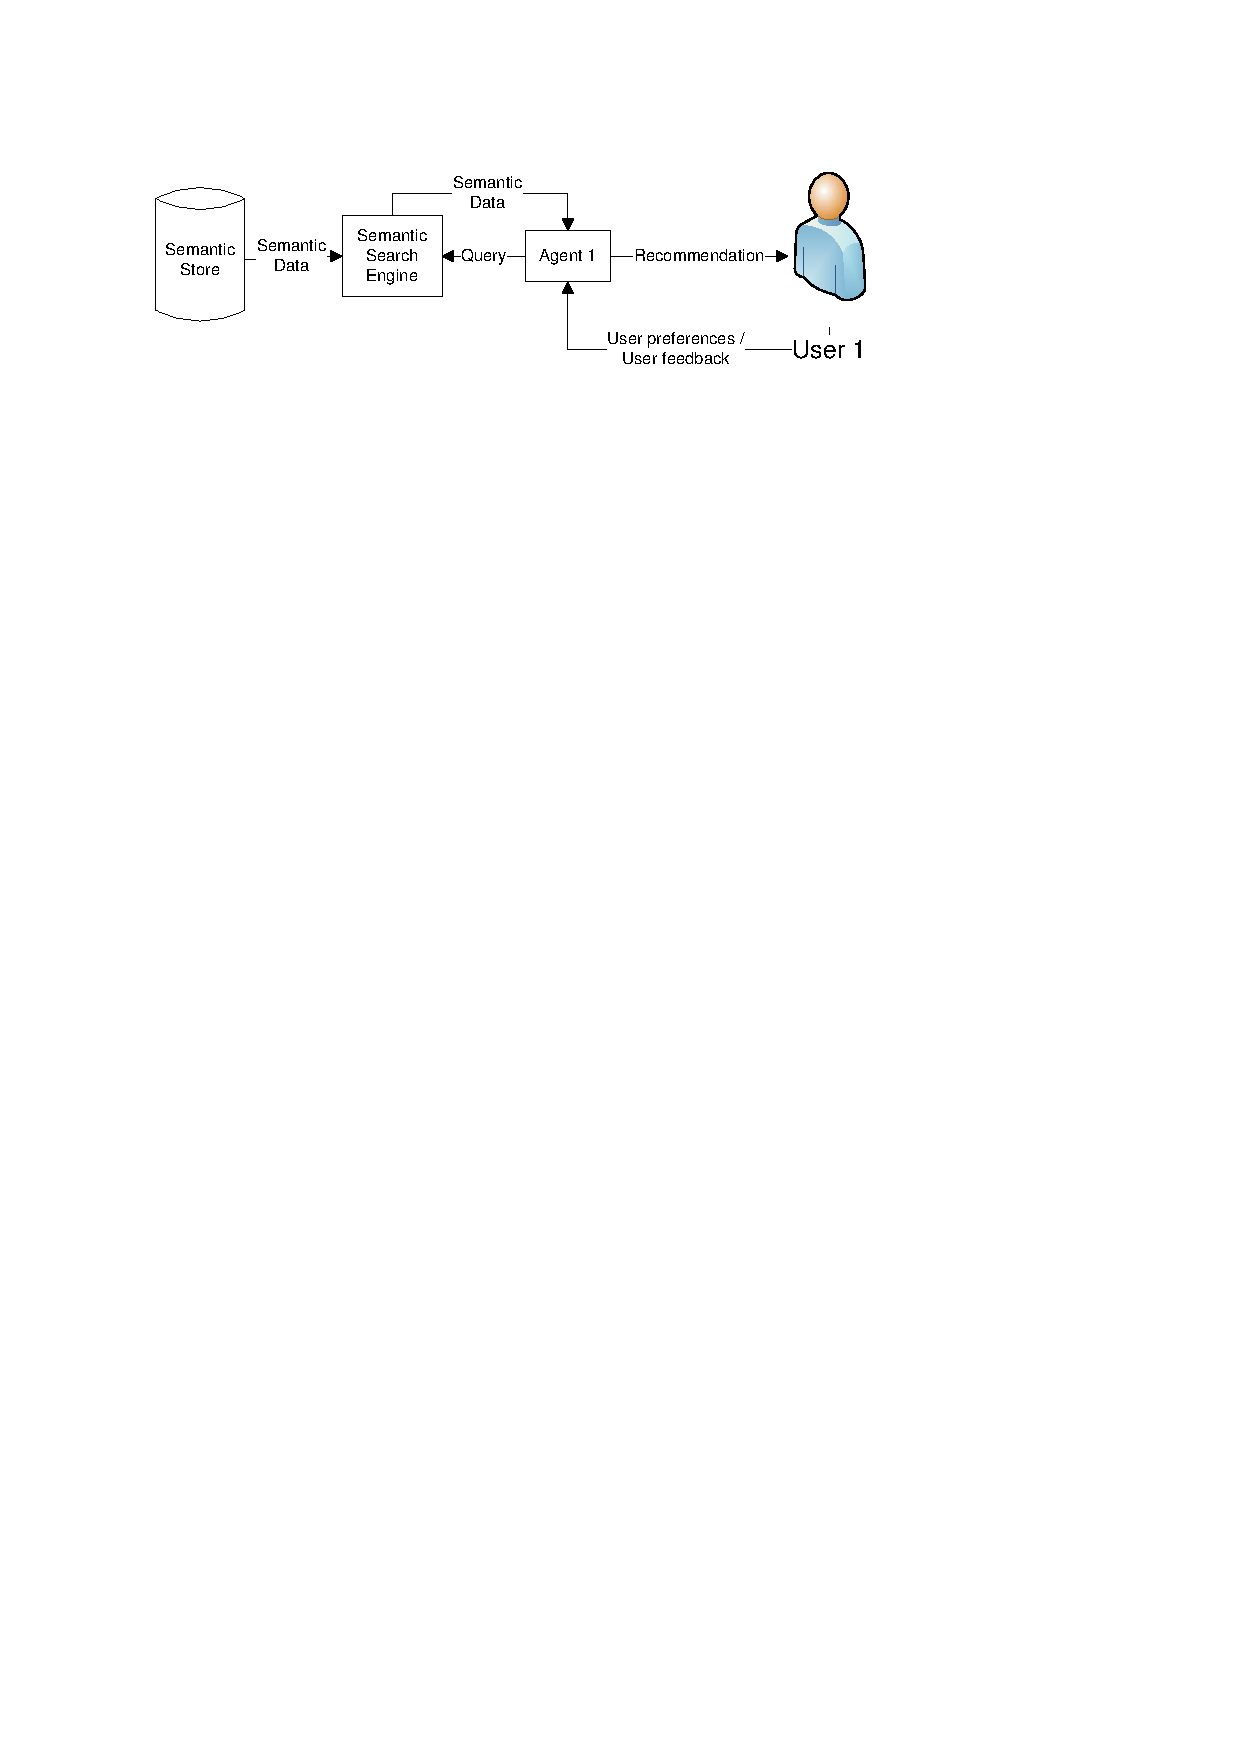
\includegraphics[width=.8\hsize]{img/UserSearch}
\caption{Process of querying Semantic Search Engine by an user agent}
\label{img:UserSearch}
\end{figure}
 
The process of a user agent searching and making use of semantic search engine is represented in Figure \ref{img:UserSearch}.

Our main focus in this paper is on the agent and on the extractors.

%\section{Egothor support for web repository}
%Egothor allows an easier retrieval of Web documents stored in the Web repository for the semantic extractors. Some functionality will be described together with the proposal of parts of our system, especially agent (Sections 5-8???). This section describes in detail and explains how Egothor runs and supports the Semantic Search engine.

%\subsection{Crawler}

%Egothor crawler is designed for high-speed efficient Web crawling. The software was implemented in Java with a strict use of NIO operations. This technology ensures high throughput (up to several MB per second on a single node) and minimizes a number of crawler fetch threads (in Figure 3 yellow parts are outside of Egothor, green filters are emphasized because of their role in our application).
 
%The central component of the crawler is a scheduler. It prepares a plan of URLs which are (re)crawled next.  The plan is affected by many factors stored in crawler's knowledge-base: network link quality, website size, number of HTTP errors during the communication with a website, history of changes in website documents in past, and other minor attributes. The knowledge-base allows the crawler to act promptly if anything (may) slow him down.

%The plan is executed by a fetch thread and then the crawled documents enter a parser. The parser is responsible to extract a next fragment of a link structure and new URLs. It also prepares SAX stream which is later analyzed by an acyclic net of filters. Each of the filters may add new tags (labels on a document) and modify the SAX stream for successive filters. The output of the filtering machinery is processed by a full-text indexer and stored in an auxiliary buffer (index chunk).  The index chunks are merged with a main index using a dynamization algorithm. Original Web documents, including the tags added by the filters, are stored in the Web repository.

%The filters must operate on the SAX stream only and cannot use any context information (who points to this page, what pages are similar, etc.) due to performance reasons. Therefore, they are able to provide a simple classification by tags like: page with HTML FRAMEs, TABLEs, real grammatical sentences (if the filter can find reasonable punctuation).


%\subsection{Web repository}
%The Egothor repository is a temporal repository of Web documents; therefore a document is identified by its id, revision number and a timestamp. The documents come together with their initial tags, and these tags can be freely modified later. The tags simplify a retrieval of documents, since you can use them instead of raw document ids and revision numbers. Moreover, the repository is also able to retrieve documents where a given Boolean formula of tags matches. The repository recognizes two tag groups: some tags are read as "for all revisions of a concrete document", while others are tied with just a given document revision.

%The architecture is based on three layers: core that saves documents and computes deltas between revisions to save space; symlink that maps core's document and revision numbers to numbers published to a user; cloud that assigns tags and manages ACL on the tags. This way the system can modify the tags without overloading the main base of raw documents.

%The repository supports document's metadata, e.g. modification and creation dates. It keeps track of all changes in a document, so that it is able to provide information about a durable (persistent) text blocks or even subtrees in DOM.





\section{Intermediate domain independent automated annotation}
Web information extraction is often able to extract valuable data. We would like to couple this process with consecutive semantic annotation (initially human trained; later it should operate automatically). In this chapter we would like to describe details of our idea to split this process in two parts - domain independent and domain dependent.

\subsection{Extraction based on structural similarity}
First approach for domain independent intermediate information extraction and semantic annotation is to use the structural similarity in web pages containing large number of table cells and for each cell a link to detailed pages. This is often presented in web shops and on pages that presents more than one object (product offer). Each object is presented in a similar way and this fact can be exploited.

As web pages of web shops are intended for human usage creators have to make their comprehension easier. Acquaintance with several years of web shops has converged to a more or less similar design fashion. There are often cumulative pages with many products in a form of a table with cells and some brief description and then there are links detailed pages to each product.

There exist many extraction tools that can process web pages like this. Most complete recent survey can be found in \cite{biblio:Chang2006} and also in \cite{biblio:WebDataMining}.  We come with similar but also different solution divided into domain dependent and domain independent phases. See below for details.
%Of course many pages of web shops belong to hidden (deep) web and require some form of initialization. Links to detailed pages can be replaced by some scripts. This can make the crawling of such pages problematic; we do not solve this problem here. Once (a part of these pages) is crawled and stored in our Egothor repository, we can process them further. 

\begin{figure}
\centering
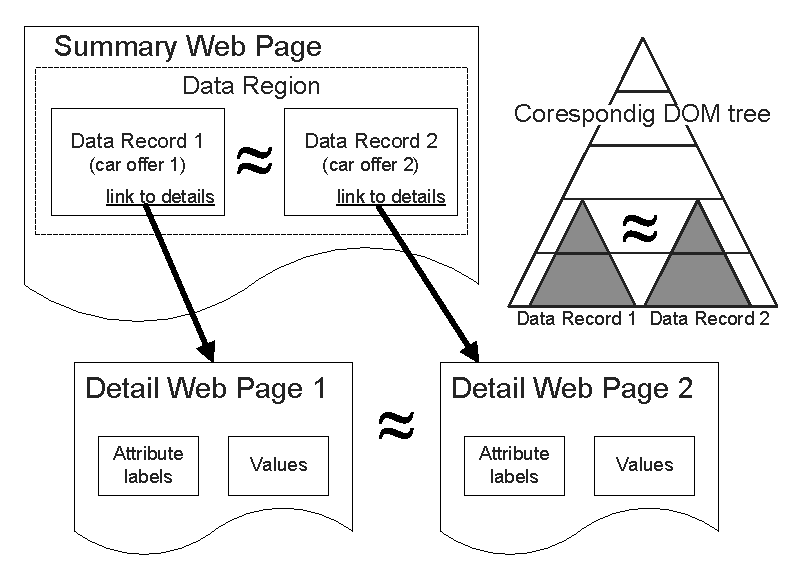
\includegraphics[width=.6\hsize]{img/StructuralSimilarity}
\caption{Structural similarity in web pages}
\label{img:StructuralSimilarity}
\end{figure}


Our main idea (illustrated in the Figure \ref{img:StructuralSimilarity}) is to use a DOM tree representation of the summary web page and by breadth first search encounter similar subtrees. The similarity of these subtrees is used to determine the data region - a place where all the objects are stored. It is represented as a node in the DOM tree, underneath it there are the similar sub-trees, which are called data records.

Our ontology engineering part is based on a bottom-up approach of building ontologies. The first classes are `tabular page', `data region' and `data record' which are connected with properties `hasDataRegion' and `hasDataRecord'. Also, between data record and its detail \emph{Data\_region} and \emph{Detailed\_page} we have property `hasDetailPage'. Note that these concepts and properties have soft computing nature which can be modeled by a fuzzy ontology. For instance, being an instance has a degree of membership depending on the precision of our algorithm (dependent on similarity measures used to detect data regions and/or records). Using some heuristics we can detect what are resources described in this page (Tabular\_page describes rdfs:Resources). To detect possible attributes and even their values we explore similarities between data record content and corresponding detailed page content. The main idea is to find same pieces of text in the data record and in the detail page. This occurs often, because a brief summary of the object is present in the data record. Somewhere near the attribute values are located the names of attributes in the detail page. These names of attributes can be extracted. The extraction of attribute names is easy because on every detail page the names will be the same.  The names of attributes can be used in our low-level ontology as names of properties - each object will be represented by the URL of the detail page, and a set of properties that consists of the attribute values found on the detail page.

This idea is modification of our previous implementation from \cite{biblio:EcHoUncertaintyIssues2008}. Here we decided to split the extraction process to the domain independent and domain dependent parts (see in section \ref{sec:ddstruct}) so the generally applicable algorithm described here is separated form the domain dependent stuff that can be supported with domain and extraction ontology (see in section \ref{sec:ddstruct}).  

%on the top of Mozilla Firefox API and experimentally tested on table pages from several domains (cars, notebooks, hotels). Tree representation was the DOM of the page, similarity between subtrees was Levenshtein editing distance (for a subtree considered as a linear string), learning thresholds for decision were trained (more see [13???]).

\begin{figure}
{\footnotesize\begin{verbatim}
1 function BFSfindDR(LevelNodes)
2 begin
3   NextLevelNodes = {}; 
4   regions = {}; 
5   for each Node in LevelNodes do 
6   begin 
7     regions=identDataRegions(normalized(Node.children)); 
8     NextLevelNodes=NextLevelNodes  U  (Node.Children not in regions);         
9   end
10    if NextLevelNodes != {}  
11      return regions U BFDfindDR(NextLevelNodes);
12    else return regions;
13 end
\end{verbatim}}
\caption{Algorithm for finding data regions on a web page}
\label{fig:alg}
\end{figure}

In the Fig.~\ref{fig:alg} is described algorithm for finding data regions. Input of the function is the root element of the DOM tree of a web page. Function BFSfindDR is recursive; each run processes one tree level. Algorithm proceeds across each node of input LevelNodes (5) and tries to identify if some of the node's children represent a data regions (7). If so, those children are excluded from further processing (8). Nodes that are not in data regions are added to NextLevelNodes. Finally, if there are some nodes in NextLevelNodes, the function is called recursively. Data regions found on the page form the output of function.
%Further improvement of annotation is left for domain dependent annotation where special extraction ontology can be trained (e.g. containing regular expressions for this special domain).

\subsection{A method based on Czech linguistics}
Our approach for Web information extraction of textual pages is based on Czech linguistics and NLP tools. We use a chain of linguistic analyzers (\cite{biblio:HajicMorfTag}, \cite{biblio:collinshbrt_1999}, \cite{biblio:KlTransformationBasedTectogrammatical2006}) that processes the text presented on a web page and produces linguistic (syntactic) trees corresponding with particular sentences. These trees serve as a basis of our semantic extraction.

Unlike the usual approaches to the description of English syntax, the Czech syntactic descriptions are dependency-based, which means that every edge of a syntactic tree captures the relation of the dependency between a governor and its dependent node. Especially the tectogrammatical (deep syntactic) level of representation \cite{biblio:MiBeAnnotationtectogrammatical2006} is closer to the meaning of the sentence. The tectogrammatical trees (Example of such a tree is on the Figure \ref{img:tectogrammatical}) have a very convenient property of containing just the type of information we need for our purpose (extraction of semantic information), namely the information about inner participants of verbs - actor, patient, addressee etc. So far this linguistic tool does not work with the context of the sentence and hence does not exploit a possible frequent occurrence of similar sentences.

\begin{figure}
\centering
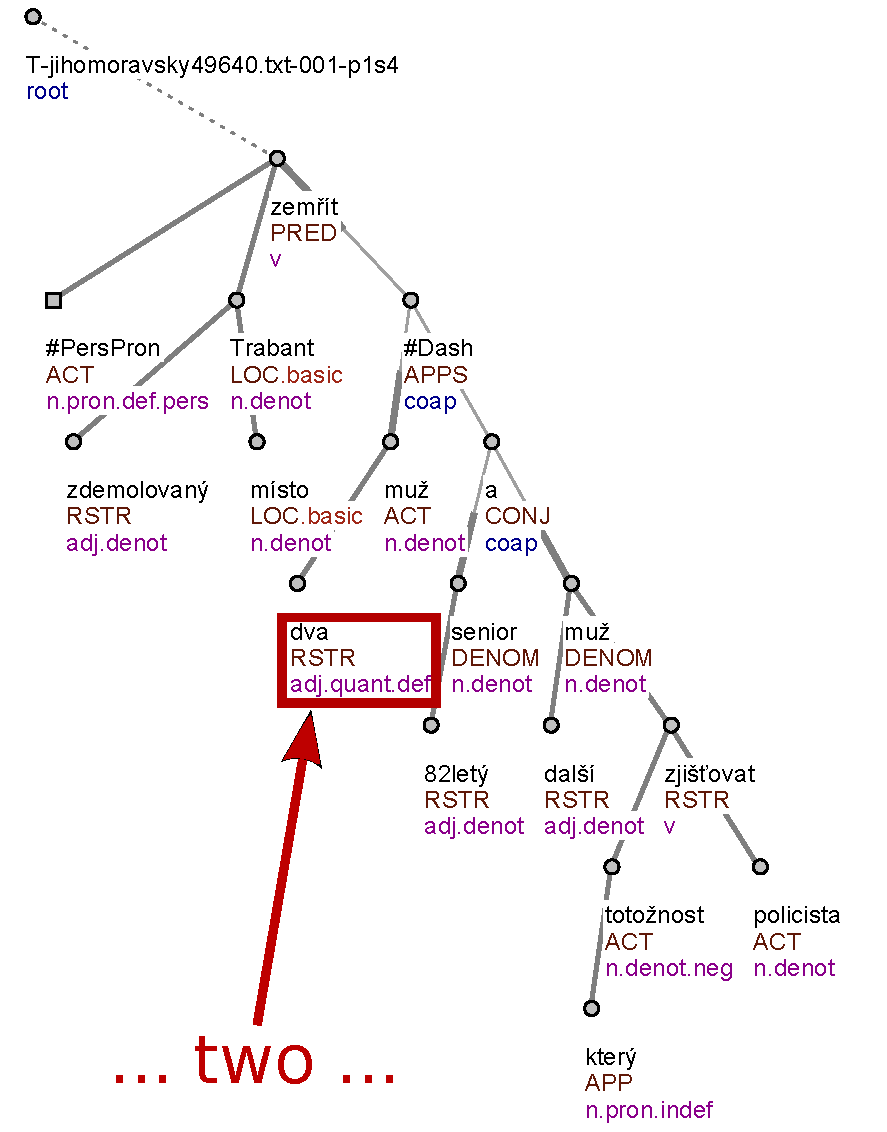
\includegraphics[width=.6\hsize]{img/TectogramaticalTree}
\caption{A tectogrammatical tree of sentence: ``Two men died on the spot in the demolished Trabant...''}
\label{img:tectogrammatical}
\end{figure}




\section{Domain dependent automated annotation}
Second phase of our extraction-annotation process is domain dependent. It makes use of previous intermediate general (domain independent) annotation. Our goal is to make this process as fast and as easy as possible, e.g. to be trained very fast (possibly in query time) and precisely by any user with average computer skills.

\subsection{Extraction and annotation based on extraction ontology} \label{sec:ddstruct}
Domain ontology is the basis for extraction ontology. Extraction ontology \cite{biblio:Embley02automaticallyextracting} extends the domain ontology by adding some additional information about how the instances of a class are presented on web pages. We used regular expressions to determine values of the properties. These regular expressions are matched against relevant pieces of text found on the web page in previous general annotation phase. These regular expressions are not dependent on an extraction tool, so the extraction ontology is general -- it contains generally applicable information, which can be shared and imported to the particular tool from variety of locations.

So far the creation of extraction ontology has to be done by a very experienced user and has to be verified on a set of web pages. In the future we plan to invest more effort and soft computing techniques in automating this part. In this paper we do not deal with learning of extraction ontology. 

%Please notice, that parts of domain ontology are properties \emph{ratioOfAccidents} and \emph{ratioOfDeath}, which have cumulative values obtained from linguistic extraction over the whole corpus. 
 
\subsection{Domain dependent annotation based on linguistics}

Assume we have pages annotated by a linguistic annotator and we have a domain ontology. The extraction method we have used is based on extraction rules. An example of such an extraction rule is on Figure \ref{img:ExtractionOntology} (on the left side). These rules represent common structural patterns that occur in sentences (more precisely in corresponding trees) with the same or similar meaning. Mapping of the extraction rules to the concepts of the target ontology enables the semantic extraction. Example of such a mapping is demonstrated in Figure \ref{img:ExtractionOntology}. This method is not limited to Czech language and can be used with any structured linguistic representation. We have published this method in \cite{biblio:DeVoComputingaggregations2008}, you con find more details there.


\begin{figure}
\centering
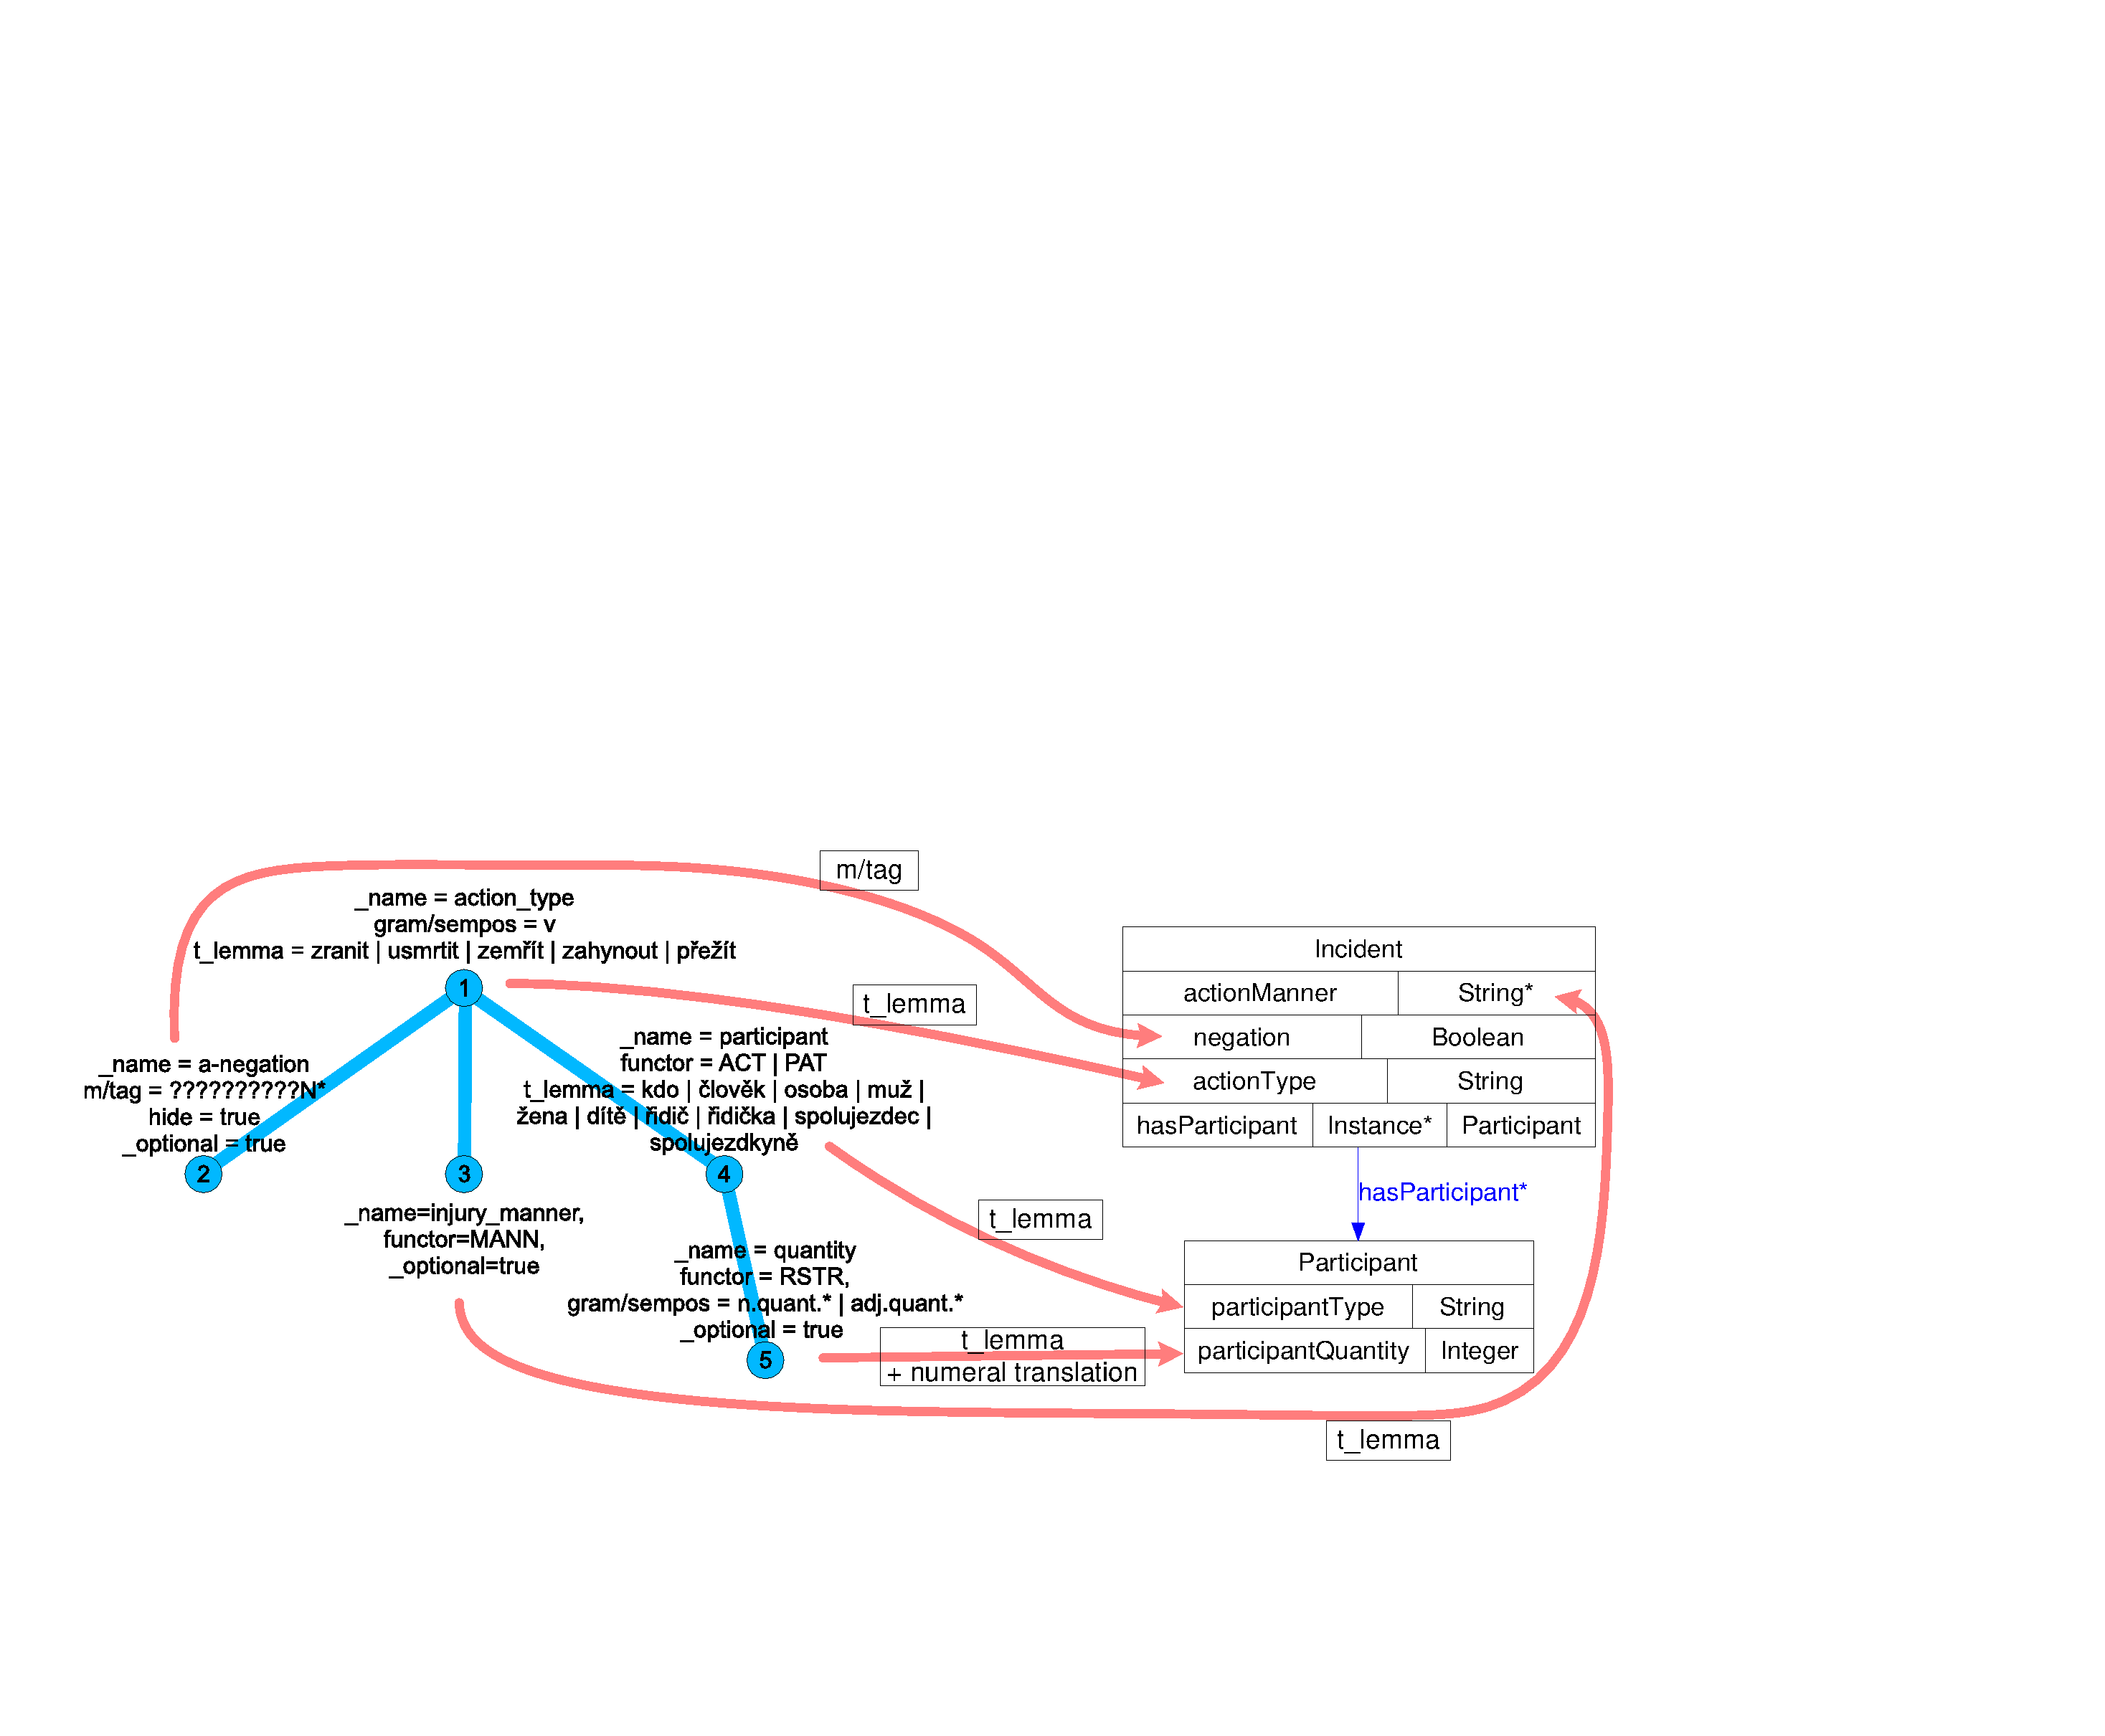
\includegraphics[width=\hsize]{img/ExtractionOntology}
\caption{An example of extraction rule and its mapping to ontology}
\label{img:ExtractionOntology}
\end{figure}

We experimented with obtaining extraction rules in two ways.
\begin{enumerate}
\item Rules and mappings were designed manually (like the rule on the Fig. \ref{img:ExtractionOntology}). 
\item Rules and mappings were learned using Inductive Logic Programming (ILP) methods (see following section).
\end{enumerate}
 Finally, having this mapping, we can extract instances of the target ontology from the answer corresponding to an extraction rule. This answer is given by the semantic repository, and the instances of the ontology are also stored there.

\subsection{Using Inductive Logic Programming (ILP)}
ILP \cite{biblio:Muggleton} is a method for a generation of rules that describe some properties of data. ILP takes three kinds of input
\begin{itemize}
	\item Positive examples E+ -- objects that have the desired property.
	\item Negative examples E- -- objects that do not have the desired property.
	\item Background knowledge -- facts about the domain (so far we do not consider background knowledge in the form of rules).
\end{itemize}

\begin{figure}
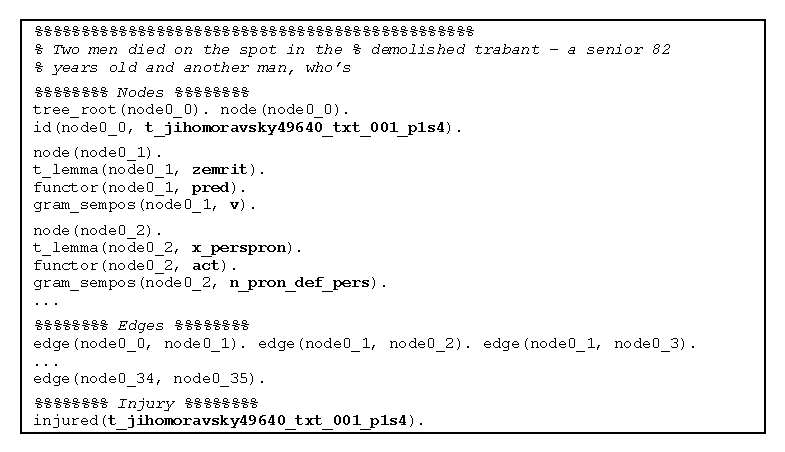
\includegraphics[width=\hsize]{img/DedEckVoj_Prolog}
\caption{Sample from prolog representation of a sentence }
\label{img:prologFacts}
\end{figure}

ILP tries to generate such rules that all positive examples and no negative example satisfy them. It uses concepts from the background knowledge in the body of the rules.
The main advantage of ILP is that it can be trained to mine arbitrary data described in predicate logic - the process of learning is dependent only on the positive and the negative examples and on the amount of information we have about them. The more information we have, the more precise the learning will be. \par

Thanks to the fact that ILP learns from positive and negative examples, we can propose an assisted learning procedure for learning and also tuning the extractor (described in previous section). The process is such that the extractor gets pure textual or semantically annotated (by the linguistic extractor) data from a web page and presents it to the user. He or she then annotates the data or only corrects the data saying which are well and which are badly annotated. The extractor can be taught and tuned to the desired goal in this way. Of course the user has to understand the semantics of the annotations - so he or she has to be an expert in that way of understanding the target ontology. Yet this ontology can be quite simple in the case we are interested only in a specific kind of information e.g. number of people injured during a car accident like in our experiments (see next section) and motivation. 

We discovered that we can use a straightforward transformation of linguistic trees (see an example on the Figure \ref{img:tectogrammatical}) to predicates of ILP (example of the transformation is in the Figure \ref{img:prologFacts}) and the learning procedure responds with significant results, which are presented in next section.

On the Figure \ref{img:tectogrammatical} we can see the relationship between particular words of a sentence and nodes of tectogrammatical tree - the highlighted node of the tree corresponds with the word `two' in the sentence (also highlighted). This relationship allows propagation of information from the user (which annotates just the text of sentence) to the ILP learning procedure.

\section{User agent}
One of the aspects of our proposed agent is to compare different offers (e.g. used car offer) based on their attributes. We call this a ``decathlon effect'', or in economy terminology utilizing possibly ``conflicting objectives''. The user has some preferences on car offer's attributes; he or she wants low price and low consumption. These preferences are called objectives. We can use fuzzy logic notation and to each attribute $A_i$ associate its fuzzy function $f_i : D_{A_{i}} \rightarrow [0,1]$, which normalizes the domain of the attribute (the higher the fuzzy value the higher the user preference).

Some of these objectives are conflicting e.g. wanting low price and low consumption. There is no clear winner, some of the car offers may be incomparable - Audi A4 has high price but also lower consumption, on the other hand Tatra T613 may have lower price but also higher consumption. Regarding two objectives ``low price'' and ``low consumption'', these two cars are incomparable.
This undecidability is solved by an aggregation function (in economy called utility function), often denoted by $@$. This function takes preference on attributes and combines them into one global score of the car offer as a whole. In this way, the agent can order all car offers by their score. The aggregation function may be a weighted average, for example:
\begin{displaymath}@(Price, Consumption)=\frac{3*Price + 1*Consumption}{4}\end{displaymath}
where $Price$ and $Consumption$ are the degrees to which the car offer satisfies the use criteria. We have spent much time in the research of user modelling, these ideas 
are discussed in detail for example in recent \cite{biblio:EcHoLearningdifferent2007}.

 
\begin{figure}
\centering
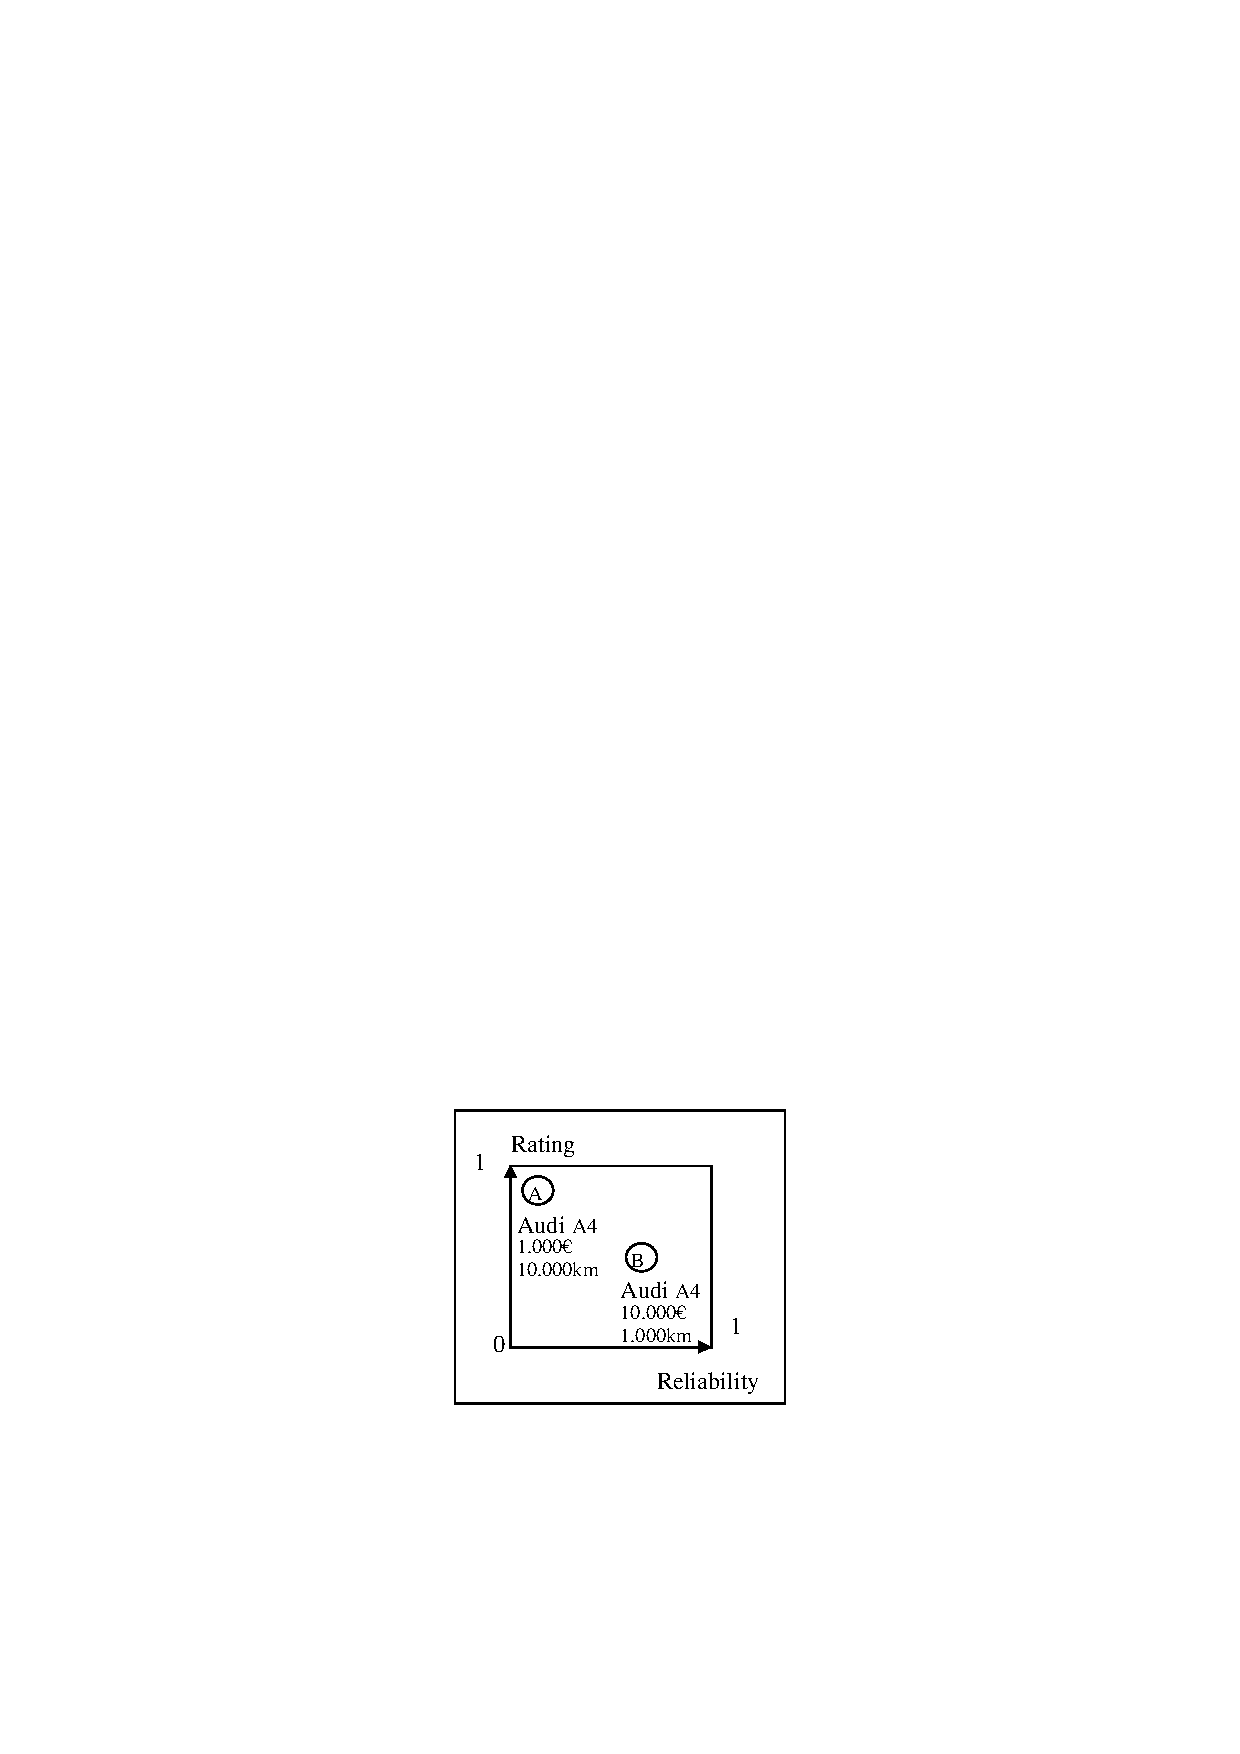
\includegraphics[width=.4\hsize]{img/CarPrefs}
\caption{An example of reliable and unreliable rating}
\label{img:rating}
\end{figure}

Another phenomenon of our approach is that we take into account the (un)certainty of correct extraction. We have in our system two information about the same offer of Audi A4. First Audi A4 denoted as $A$ has much higher rating than the same Audi denoted as $B$ in the example in Fig.~\ref{img:rating}. However, $A$ has also much lower reliability. The reliability of the rating of $A$ and $B$ is determined by extractors that made the annotation or by later user feedback, finding first extractor mistaken. This may be caused for example by an error of extractor that switched the price (10.000(Euro)) with the distance travelled (1.000(km)). Thus $A$ has much better price than $B$ and consequently also the rating. 
We use a second order utility function to combine preference degree and reliability trained to specific user profile.

\section{Experiments}
Our experiment was to enable our agent to access semantic information from the web. We tried to gather information form car offers with information about car accidents. We wanted to find out the number of injured persons during car accidents and match them to the offers according the car make and model. We have used firemen reports; some of them were about car accidents, some were not. Each report was split into sentences and each sentence was linguistically analyzed and transformed into a tectogrammatical tree, as described above. These trees were transformed to a set of Prolog facts (see Figure \ref{img:prologFacts}). \par
Sentences, which talk about an injury during a car accident, were manually tagged by predicate \verb#injured(X)#, where X is the ID of the sentence. Those sentences that do not talk about injured persons during a car accident were tagged as \verb#:-injured(X)#, which represents a negative example. This tagging can be done even by a user unexperienced in linguistics and ILP, but he or she has to understand the semantics of information he is tagging (in usually means that he or she has to understand the target ontology).
These tagged sentences were the input for ILP, we have used 22 sentences as positive examples and 13 sentences as negative examples.
We used Progol \cite{biblio:Muggleton2} as ILP software.
The rules ILP found are in following Figure \ref{img:rules}.

\begin{figure}
{\footnotesize
\begin{verbatim}
injured(A) :- id(B,A), id(B,t_57770_txt_001_p5s2).
injured(A) :- id(B,A), id(B,t_60375_txt_001_p1s6).
injured(A) :- id(B,A), id(B,t_57870_txt_001_p8s2).
injured(A) :- id(B,A), id(B,t_57870_txt_001_p1s1).

injured(A) :- id(B,A), edge(B,C), edge(C,D), t_lemma(D,zranit).         
injured(A) :- id(B,A), edge(B,C), edge(C,D), t_lemma(D,nehoda).
\end{verbatim}}
\caption{Rules mined by ILP}\label{img:rules}
\end{figure}

The first four rules are overfitted to specific sentences. Only the last two represent generally applicable rules. But they do make sense - `zranit' means `to hurt' and `nehoda' means `an accident' in Czech. These two rules mean that the root element is connected either to a noun that means an accident or to a verb that means to hurt.\par
We tested these rules on the set of 15 positive and 23 negative examples. The result accuracy was 86.84\%.
%Detailed results are in Fig.~\ref{fig:results}.
%P is the positive sentence from ILP, ~P is negative sentence, A is sentence tagged as positive and $\neg$A is sentence tagged as negative. 11 sentences that were tagged as positive by the user were also tagged as positive by ILP, 4 was tagged as negative by ILP. 22 sentences that were tagged as negative by the user were also tagged as negative by ILP, only 1 was tagged as positive by ILP.


%\begin{figure}
%\label{fig:results}
%\centering
%\begin{tabular}{|c|c|c|} \hline
% 		&A	&$\neg$A	\\ \hline
%P		& 11&1 \\ \hline
%$\neg$P	& 4 &22\\ \hline
%\end{tabular}
%\caption{Results on the test set}
%\end{figure}


In this case we learned a set of rules that identifies relevant sentences -- roots of relevant tectogrammatical trees. We have made some additional experiments (some of them were published in \cite{biblio:DeEcExperimentswith2008}) that seems to lead to our goal. It is still a long way to go, but we understand these results as a proof of concept that ILP can be used for finding different kinds of information present in nodes and structure of linguistic trees. We for example extracted number of injured people from relevant trees when we have modified the training data. And still there is the possibility to design extraction rule manually if the learning method fails.

\section{Conclusions and further work}
In this paper we have developed the idea of web semantization, which can help to arch over the gap between Web of today and Semantic Web. We have presented a proof of concept that even today it is possible to develop a semantic search engine designed for software agents. % in the scale of *.cz pages.
In particular contributions consists of two sorts of automated third party annotation of existing web resources, the idea of a semantic repository serving as a sample of semantized web with extension of the ontology model for additional annotation (e.g. uncertainty annotation) and a proposal of an intelligent agent.\par
Future work goes in two directions. First is in the integration of specific parts of the system,  in the automation of the whole process and in the extensive experiments with a larger number of different users. Second is in improving special parts of the system - either making it more precise or making it more automatic (able to train by a less qualified user).

%ACKNOWLEDGMENTS are optional
\subsection{Acknowledgments}
This work was partially supported by Czech projects 1ET100300517, 201/09/0990 GA�R and MSM-0021620838.
%
% The following two commands are all you need in the
% initial runs of your .tex file to
% produce the bibliography for the citations in your paper.

\bibliographystyle{splncs}
\bibliography{ESWC_webSemantization}  % sigproc.bib is the name of the Bibliography in this case

\end{document}
